\documentclass[11pt]{article}
\renewcommand{\baselinestretch}{1.05}
\usepackage{amsmath,amsthm,verbatim,amssymb,amsfonts,amscd, graphicx}
\usepackage{blindtext}

\usepackage{caption}
\usepackage{enumitem}

%Additional Packages
\usepackage{enumitem}
\usepackage{graphics}
\usepackage{float}
\graphicspath{ {images/} }
%\usepackage[framed]{mcode}
\usepackage{hyperref}
\hypersetup{
	colorlinks=true,
	linkcolor=blue,
	filecolor=magenta,      
	urlcolor=cyan,
}

\topmargin0.0cm
\headheight0.0cm
\headsep0.0cm
\oddsidemargin0.0cm
\textheight23.0cm
\textwidth16.5cm
\footskip1.0cm
\theoremstyle{plain}
\newtheorem{theorem}{Theorem}
\newtheorem{corollary}{Corollary}
\newtheorem{lemma}{Lemma}
\newtheorem{proposition}{Proposition}
\newtheorem*{surfacecor}{Corollary 1}
\newtheorem{conjecture}{Conjecture} 
\newtheorem{question}{Question} 
\theoremstyle{definition}
\newtheorem{definition}{Definition}

\usepackage{indentfirst}
%\renewcommand{\thesubsubsection}{\thesubsection.\alph{subsection}}

\newcommand{\floor}[1]{\lfloor #1 \rfloor}

%SETUP PSUEDOCODE
\usepackage{tcolorbox}


%SETUP AtxMEGA128A1U
\usepackage{listings}

\usepackage{xcolor}
\definecolor{bluekeywords}{rgb}{0.13,0.13,1}
\definecolor{greencomments}{rgb}{0,0.5,0}
\definecolor{turqusnumbers}{rgb}{0.17,0.57,0.69}
\definecolor{redstrings}{rgb}{0.5,0,0}

\lstdefinelanguage{atxmega128a1u}{
	morekeywords={include, ,org, rjmp, CSEG, db, equ, DSEG, ldi, lds, sts,  breq, brne, and, cp, cpi, push, pop, ret},
	keywordstyle=\color{bluekeywords},
	sensitive=false,
	morecomment=[l][\color{greencomments}]{;},
	morecomment=[s][\color{greencomments}]{{/*}{*/}},
	morestring=[b]",
	stringstyle=\color{redstrings}
}

\lstnewenvironment{asmlisting}{
	\lstset{
		frame=single,
		language=atxmega128a1u,
		basicstyle=\ttfamily,
		breaklines=true,
		columns=fullflexible
	}
}
{}
%
% START OF DOCUMENT
%
\begin{document}
\captionsetup[figure]{labelfont=bf} 

\title{Lab 2}
\author{\textbf{Michael Arboleda}\\Lab Section: 7F34}
\maketitle
%
% PRELAB QUESTIONS
%
\section*{b. Answers to all pre-lab questions}
\begin{enumerate}[label={\arabic*)},font={\color{red}\bfseries}]
	%
	%1
	%
	\item What is the default clock frequency of the XMEGA?
	\\[0.8ex]
	\textbf{ANS:} The default clock frequency of the XMEGA is 2MHz
	.
	%
	%2
	%
	\item What would you need to do to run the XMEGA at 16 MHz?
	\\[0.8ex]
	\textbf{ANS:} To run the XMEGA at 16 MHz would need to set the clock to 32MHz and then divide by 2 using a prescaler
	.
	%
	%3
	%
	\item The XMEGA is rated to run at frequencies up to 32 MHz, but some peripherals run up to either 2x or 4x of this frequency. How can the XMEGA be configured to run at 32 MHz, the 2x peripheral clock at 64 MHz, and the 4x peripheral clock at 128 MHz without using any external clock sources? 
	\\[0.8ex]
	\textbf{ANS:}
	One way to get values higher than 32MHz is to use PPL. PPLCTRL, the PPL control register allows to set a multiplication factor. This includes values from time 1 to times 31. Thus if 64MHz and 128MHz are need, the PPL would have to be set to time 2 and times 4 respectively.
	%
	%4
	%
	\item Why are timers useful? 
	\\[0.8ex]
	\textbf{ANS:}  Timers are useful because they are more accurate than software delays . They work in tandem with the processor’s clock. The timers in ATxMEGA provide accurate programming execution timing, thus making a programs timing accurate, which is important to time-sensitive programs.
\end{enumerate}
%
% PROBLEMS ENCOUNTERED
%
\section*{c. Problems Encountered}
I could not get my clock frequency to output. This was because I did not use a dirset to make the port an output 
%
% FUTURE WORK
%
\section*{d. Future Work/Applications}
After finishing the lab it is clear that there is much that can be done. I am interested in making a program that cycles through all the colors that the LED can make.  
%
% SCHEMATICS
%
\section*{e. Schematics}
N/A
%
% PSEUDOCODE
%
\newpage
\section*{g. Pseudocode/Flowcharts}
%
% PSEUDOCODE PART A
%
\textbf{\textcolor{blue}{Pseudocode for lab2a.asm:}}
\begin{tcolorbox}
\begin{verbatim}
MAIN:

* Equate numbers
* Set registers to hold constants
* Call Change_CLK_4HZ subroutine

WHILE(true){}
END


SUBROUTINE Change_CLK_4HZ
    * Enable the new oscillator

WHILE(32Hkz OSC FLAG not set){}

    * Write the “IOREG” signature to the CPU_CCP reg
    * Select the new clock source in the CLK_CTRL reg
    * Write the “IOREG” signature to the CPU_CCP reg
    * Set Prescalar
    * Set clock output to port c
	* Return to program
\end{verbatim}
\end{tcolorbox}
%
% PSEUDOCODE PART B
%
\newpage
\textbf{\textcolor{blue}{Pseudocode for lab2b.asm:}}
\begin{tcolorbox}
\begin{verbatim}
MAIN:

* Equate numbers
* Set registers to hold constants
* Set Port F to write
* Set TOP value for counter
* Set Prescalar for counter

WHILE(TRUE){
    * Output counter value
}
\end{verbatim}
\end{tcolorbox}	
%
% PSEUDOCODE PART C
%
\newpage
\textbf{\textcolor{blue}{Pseudocode for lab2c.asm:}}
\begin{tcolorbox}
\begin{verbatim}
MAIN:

* Equate numbers
* Set registers to hold constants

* Call Change_CLK_32HZ subroutine
* Set TOP value for counter
* Set Prescalar for counter
* Set Port D to write

WHILE(TRUE){
    if(Counter is 0){
        * Turn all lights on
    }
    if(Counter equals red max time){
        * Turn Red LED Off
    }
    if(Counter equals green max time){
        * Turn Green LED Off
    }
    if(Counter equals blue max time){
        * Turn Blue LED Off
    }
}

END


SUBROUTINE Change_CLK_4HZ
   * Enable the new oscillator

    WHILE(OSC FLAG not set){}

    * Write the “IOREG” signature to the CPU_CCP reg
    * Select the new clock source in the CLK_CTRL reg
    * Return to program

\end{verbatim}
\end{tcolorbox}

\newpage
\section*{h. Program Code}
\textbf{\textcolor{blue}{Code for lab2a.asm:}}
\lstinputlisting[language=atxmega128a1u, frame=single]{lab2a.asm}
\newpage
\textbf{\textcolor{blue}{Code for lab2b.asm:}}
\lstinputlisting[language=atxmega128a1u, frame=single]{lab2b.asm}
\newpage
\textbf{\textcolor{blue}{Code for lab2c.asm:}}
\lstinputlisting[language=atxmega128a1u, frame=single]{lab2c.asm}
\section*{i. Appendix}
\begin{figure}[H]
	\centering
	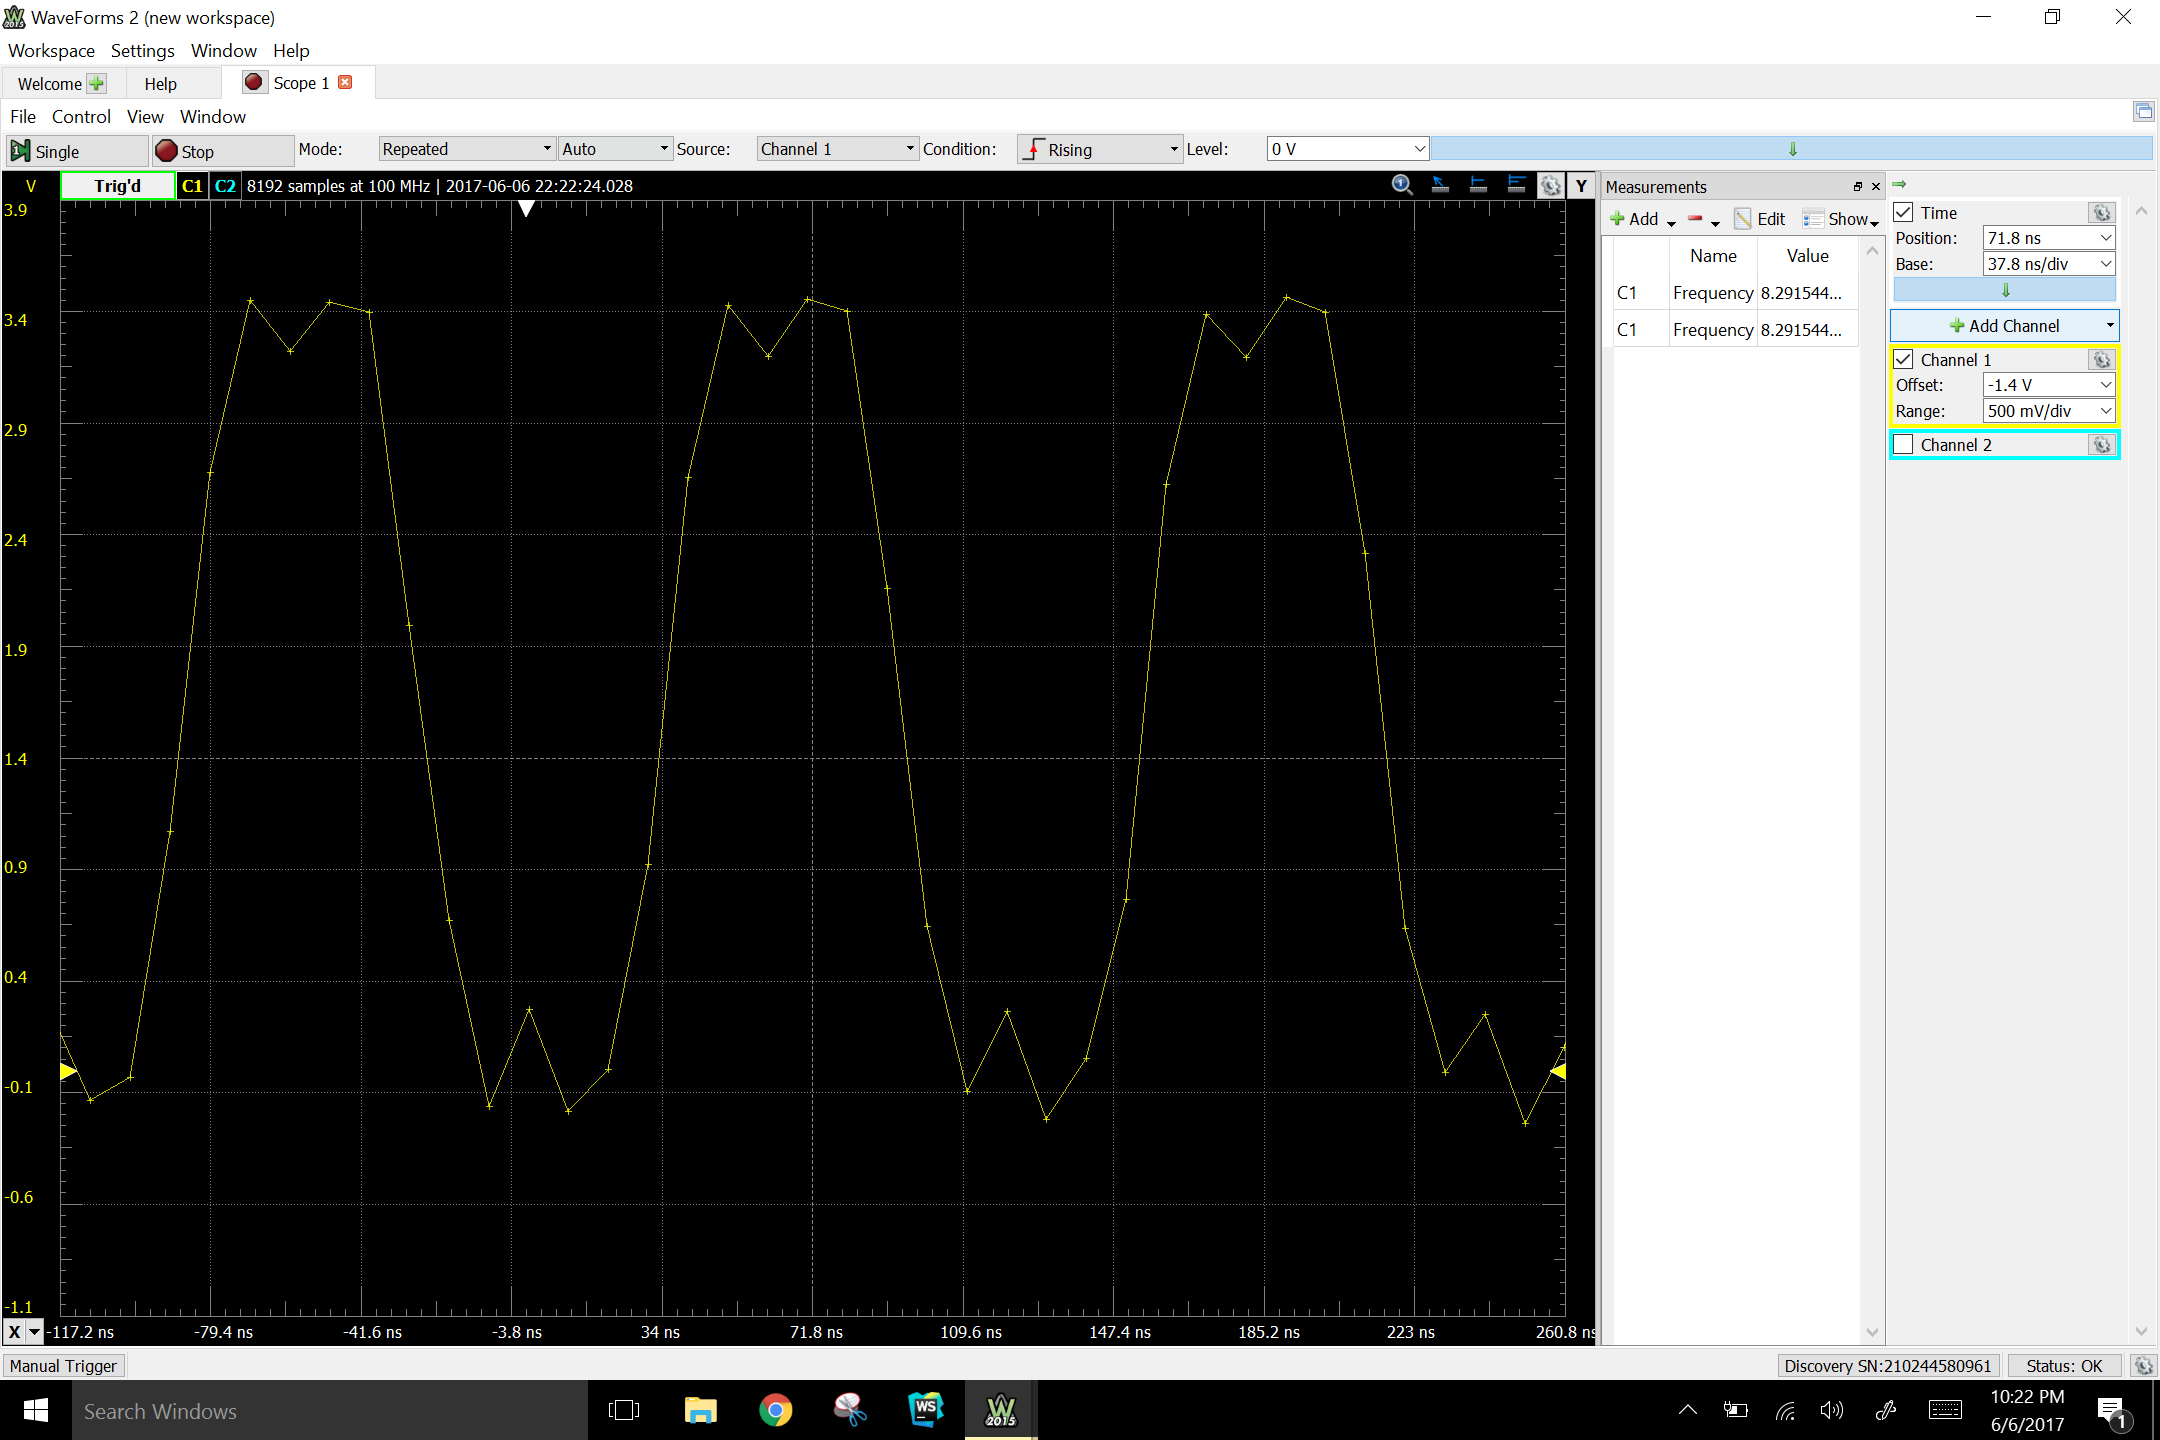
\includegraphics[width=\textwidth]{2a8mhz}
	\label{fig:a0}
	\caption{PART A: Clock at 8 MHz}
\end{figure}
\begin{figure}[H]
	\centering
	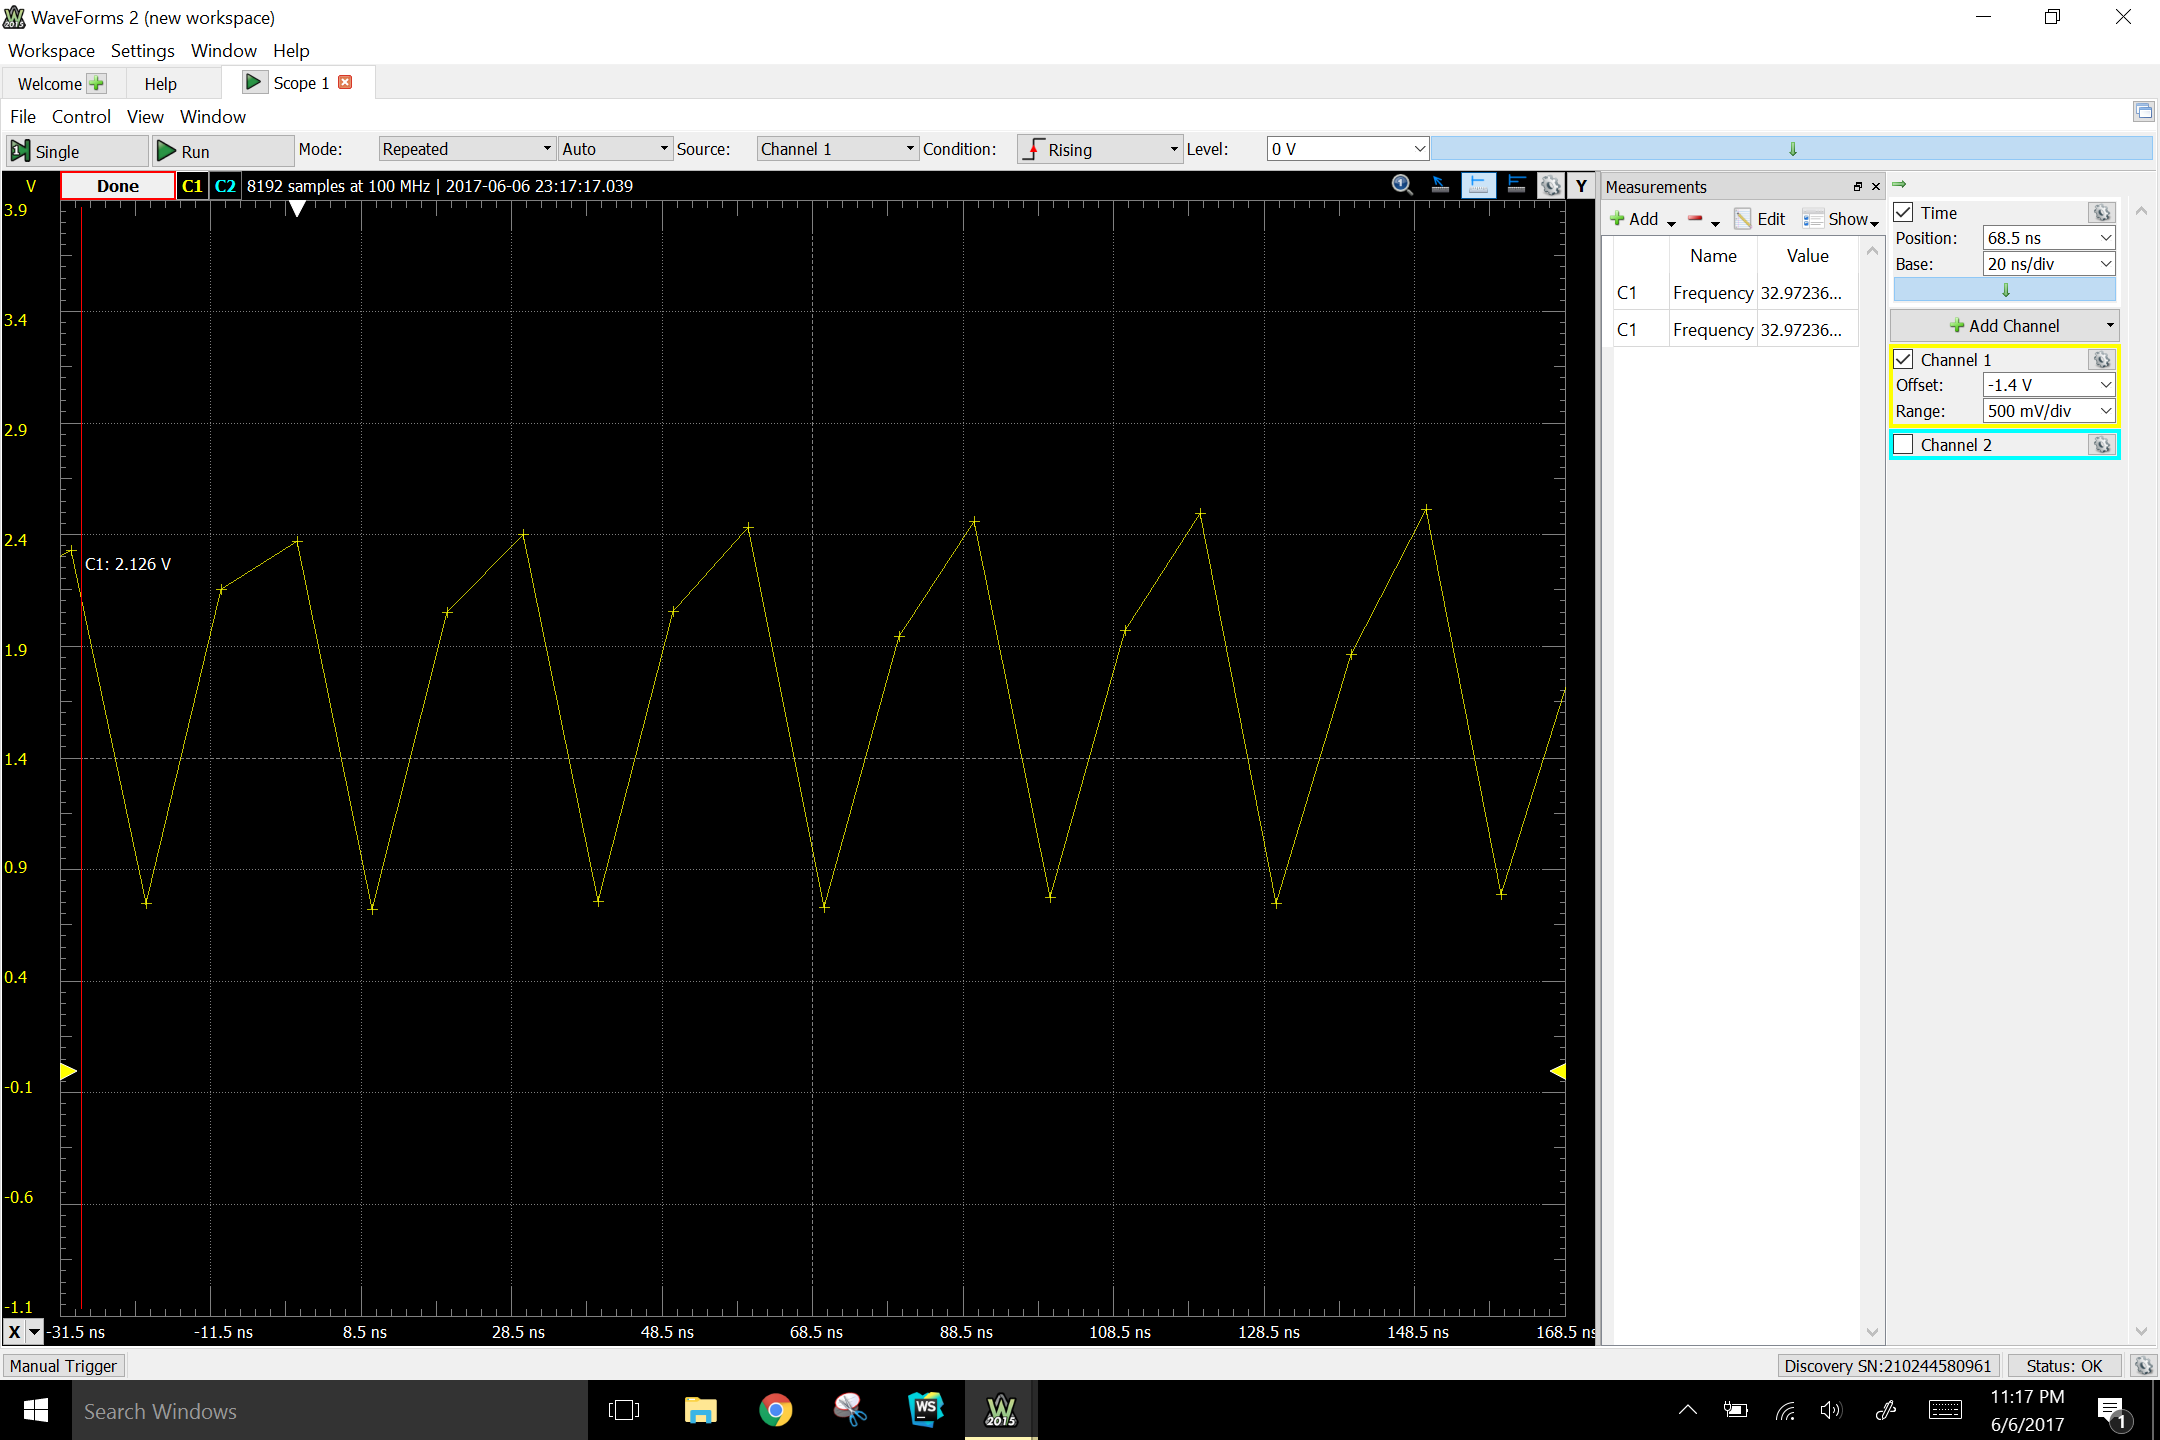
\includegraphics[width=\textwidth]{2a32mhz}
	\label{fig:a1}
	\caption{PART A: Clock at 32 MHz}
\end{figure}
\begin{figure}[H]
	\centering
	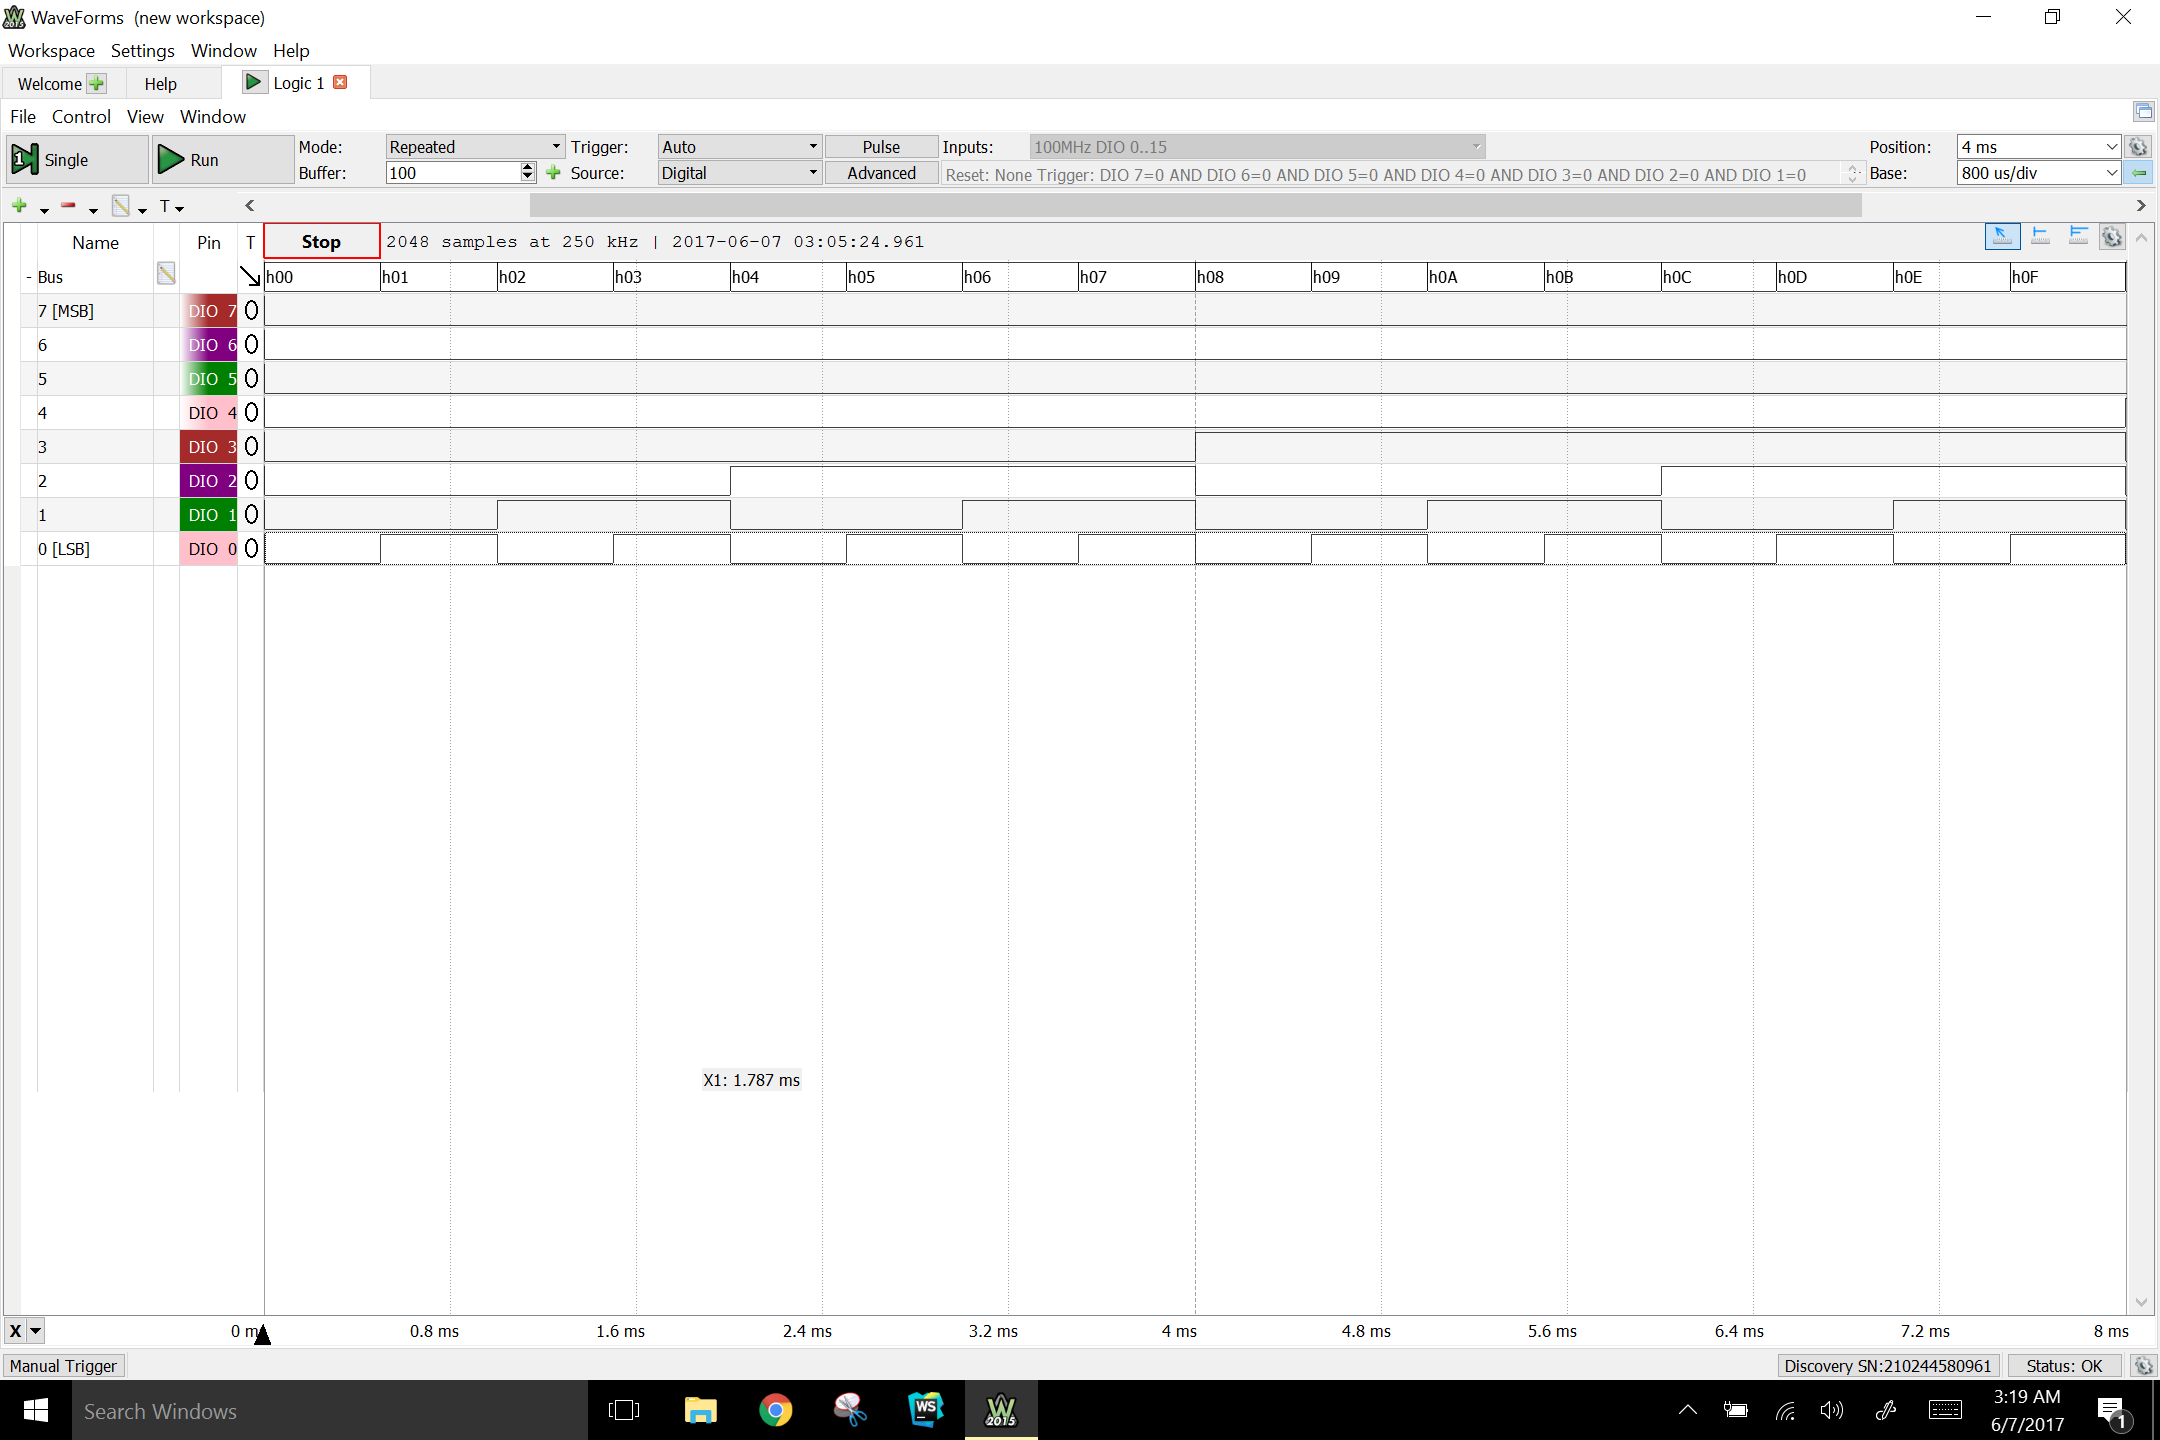
\includegraphics[width=\textwidth]{2b}
	\label{fig:c}
	\caption{PART B: Counter (0-F)}
\end{figure}
\textbf{LED Values}\\
20-0-0: A pink Light\\
80-0-0: A red light. Not that bright\\
FF-0-0: A very bright red light\\
0-FF-0: A very bright green light\\
FF-FF-0: A very bright yellow light
\end{document}